\documentclass[UTF8,a4paper,10pt]{ctexart}
\usepackage[left=2.50cm, right=2.50cm, top=2.50cm, bottom=2.50cm]{geometry} %页边距
\CTEXsetup[format={\Large\bfseries}]{section} %设置章标题居左
 
 
%%%%%%%%%%%%%%%%%%%%%%%
% -- text font --
% compile using Xelatex
%%%%%%%%%%%%%%%%%%%%%%%
% -- 中文字体 --
%\setmainfont{Microsoft YaHei}  % 微软雅黑
%\setmainfont{YouYuan}  % 幼圆    
%\setmainfont{NSimSun}  % 新宋体
%\setmainfont{KaiTi}    % 楷体
%\setmainfont{SimSun}   % 宋体
%\setmainfont{SimHei}   % 黑体
% -- 英文字体 --
%\usepackage{times}
%\usepackage{mathpazo}
%\usepackage{fourier}
%\usepackage{charter}
\usepackage{helvet}
 
 
\usepackage[colorlinks,linkcolor=black, anchorcolor=green, citecolor=black]{hyperref} 
\usepackage{amsmath, amsfonts, amssymb} % math equations, symbols
\usepackage[english]{babel}
\usepackage{color}      % color content
\usepackage{graphicx}   % import figures
\usepackage{url}        % hyperlinks
\usepackage{bm}         % bold type for equations
\usepackage{multirow}
\usepackage{booktabs}
\usepackage{epstopdf}
\usepackage{epsfig}
\usepackage{algorithm}
\usepackage{algorithmic}
\renewcommand{\algorithmicrequire}{ \textbf{Input:}}     % use Input in the format of Algorithm  
\renewcommand{\algorithmicensure}{ \textbf{Initialize:}} % use Initialize in the format of Algorithm  
\renewcommand{\algorithmicreturn}{ \textbf{Output:}}     % use Output in the format of Algorithm  

\usepackage{tabularx}   
\usepackage{tcolorbox}
\usepackage{listings}
\usepackage{xcolor}
\lstset{
    numbers=left, 
    numberstyle= \tiny, 
    keywordstyle= \color{ blue!70},
    commentstyle= \color{red!50!green!50!blue!50}, 
    frame=shadowbox, % 阴影效果
    rulesepcolor= \color{ red!20!green!20!blue!20} ,
    escapeinside=``, % 英文分号中可写入中文
    xleftmargin=2em,xrightmargin=2em, aboveskip=1em,
    framexleftmargin=2em
} 



\usepackage{fancyhdr} %设置页眉、页脚
\pagestyle{fancy}
\lhead{}
\chead{<<自然语言处理>>实验报告}
%\rhead{\includegraphics[width=1.2cm]{fig/ZJU_BLUE.eps}}
%\lfoot{}
%\cfoot{}
%\rfoot{}
 
 
%%%%%%%%%%%%%%%%%%%%%%%
%  设置水印
%%%%%%%%%%%%%%%%%%%%%%%
%\usepackage{draftwatermark}         % 所有页加水印
%\usepackage[firstpage]{draftwatermark} % 只有第一页加水印
% \SetWatermarkText{Water-Mark}           % 设置水印内容
% \SetWatermarkText{\includegraphics{fig/ZJDX-WaterMark.eps}}         % 设置水印logo
% \SetWatermarkLightness{0.9}             % 设置水印透明度 0-1
% \SetWatermarkScale{1}                   % 设置水印大小 0-1    
 
\usepackage{hyperref} %bookmarks
\hypersetup{colorlinks, bookmarks, unicode} %unicode
 
\usepackage{pdfpages}
 
\title{\textbf{基于Transformer的机器翻译}}
\author{ 贾栋 \thanks{Blog: https:kobehub.github.io} }
\date{\today}
 
\begin{document}
\includepdf[pages={1}]{page.pdf}
\maketitle
 
%\begingroup
%\color{black}
%\renewcommand{\contentsname}{目录}
%\tableofcontents
%\newpage
%\endgroup

%\begin{abstract}
%这是一篇中文小论文。这个部分用来写\href{https:kobehub.github.io}{\color{blue}摘要}。摘要的章标题默认是英文,还没找到改成中文的方法:(
%\end{abstract}
 
 
\section*{一、实验目标}
本次自然语言处理课程实验的主要任务有以下两个.

首先是基于现有研究成果,实现一个英译中的机器翻译引擎,可以提供英译
中 的 基 本 API 。 利 用 实 验 提 供 的 UMCORPUS 数 据 集 以 及 其 他 的 一 些 开 源 数 据 集
(OpenSubtitles、OpenUN、WMT18)进行训练。实验的初始目标是基于论文\href{https://arxiv.org/pdf/1808.09381.pdf}{\color{blue}Transformer Big + BT (Edunov et al., 2018)} (英德互译),
中所提出的 Transformer+BT 模型进行实现,最终只实现了
Transformer 的基础模型,用于完成英译中的翻译任务。

其次是从机器翻译的基本方法出发,我们选取了能够代表三大主流方法的开源模型的进行了模型的本地化以及对比,主要有以下模型:

\begin{itemize}

\item[$$$\bullet$] \href{http://www.statmt.org/moses/?n=Moses.Overview}{\color{blue}\underline{Mose}}  基于统计的 

\item[$\bullet$] \href{https://github.com/apertium}{\color{blue}\underline{Apertium}}                基于规则的

\item[$\bullet$] \href{http://thumt.thunlp.org/}{\color{blue}\underline{THUMT}}                     基于神经网络的
\end{itemize}
 
 利用以上模型,基于同一个数据集进行性能测试,比较不同的方法的优缺点。同时,对于在Transformer模型实现过程中的问题进行改进。
\setcounter{section}{2}
 \section*{二、实验环境}

\subsection{开发环境}
\begin{itemize}
  \item 操作系统: Arch Linux
  \item 编辑器:   vim
  \item 文档:     \LaTeX, Markdown
\end{itemize}

\subsection{运行环境}

\begin{itemize}
  \item 操作系统: Linux GPU-Server
  \item cuda: 10.0
  \item cudnn: 7.0
  \item python 3.6
  \item tensorflow-1.13.0
  \item keras-2.2.4
  \item numpy-1.15.4
  \item scipy-1.1.0
  \item scikit-learn0.20.0
  \item scikit-image0.12.3
  \item torch-1.0.0
\end{itemize}

\setcounter{section}{3}
\section*{三、原理和模型论述}

\setcounter{subsection}{0}
\subsection{原理介绍}
  实验使用 Transformer 模型进行序列化翻译的任务。有关实验原理,从基本的
Attention 机制,Multi-Headed Attention、Self-Attention 三个方面进行阐述。
\subsubsection{Attention Mechanism}
Attention 机制最早应用于图像领域,从开始的添加了 Attention 的基于 RNN 的图
像分类,到利用 Attention 机制在机器翻译任务上将翻译以及对齐同时进行的首次
NLP 尝试。Attention 机制被逐渐广泛应用在基于 CNN/RNN 等神经网络模型的 NLP
任务中去。Attention 机制灵感来源于人类的视觉系统,视觉系统进行感知时,不
会将一个场景从头到尾全部扫描,而是根据需求,着重观察感兴趣的部分。实际使
用时就是不同的权重参数,得到的一个加权和。

    \centerline{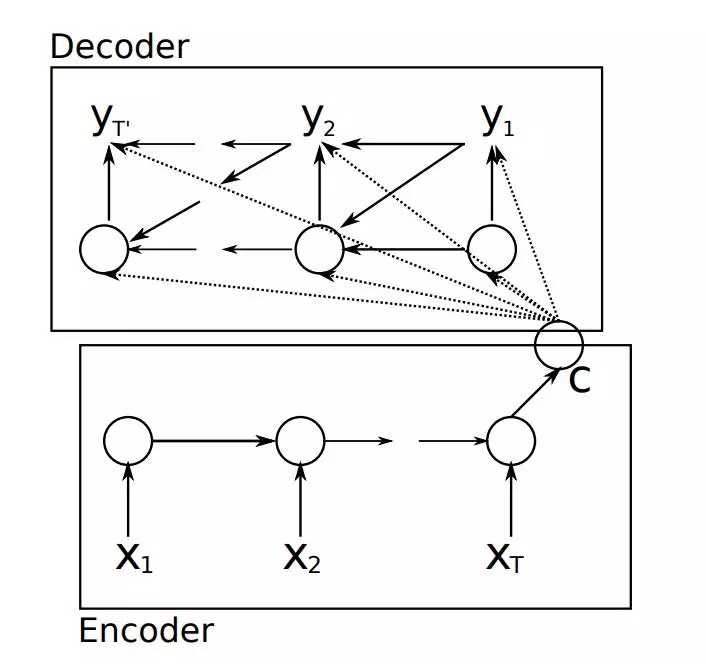
\includegraphics[scale=0.3]{pics/190417-s1.jpg}}
从一个基础的 Seq2seq 模型出发,如上图所示。对于机器翻译任务,可以抽象为\textbf{如
何把一个变长的输入序列映射为一个变长的输出序列}。其中 Encoder 把输入的 T 维向
量编码为一个固定长度的隐向量 c(或者称为上下文向量 context),其作用有二:初
始化 Decoder 模型,作为背景向量指导序列中每一步 $y_t$ 的输出。Decoder 通过每一
步的背景向量以及上一步的状态 $y_{_{}t-1}$ 得到时刻 $t$ 的输出 $y_t$,直到序列结束(<EOS>)。

但是基础的Seq2seq模型对于输出序列x缺乏区分度,所以加入的Attention机制,下图是\href{https://arxiv.org/abs/1409.0473}{\color{blue}Bahadanau attention}的示意图:
    
    \centerline{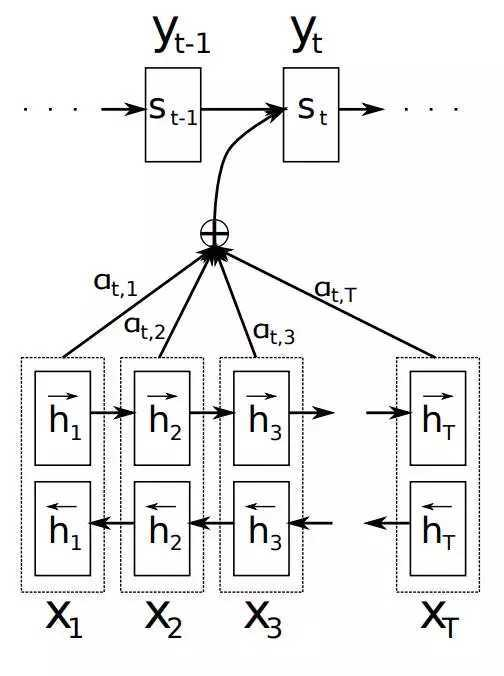
\includegraphics[scale=0.3]{pics/190417-s3.jpg}}
    
    
   该模型中定义了一个条件概率:

    \centerline{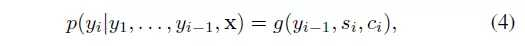
\includegraphics[scale=0.6]{pics/190417-s2.jpg}}
    
    首先将输入序列$X =(x_0, x_1, ...,x_T)$ 映射到一个隐含层状态$H=(h_0, h_1, ...,h_T)$,再由Decoder将隐层 $H$,映射到输出序列$Y=  (y_0, y_1, ...,y_t)$.这里的精妙之处在于,通过 attention 机制,输出序列Y的每一个元素都与隐层状态H相连,而H又与所有的输入状态存在联系,所以可以直接建立长距离的依赖,发掘更多语义上的关联,从而达到更好的翻译效果。

    \textbf{使用Attention机制的计算过程:}
      \begin{itemize}
        \item  使用$h$表示Encoder的隐含状态,$s​$表示Decoder 的隐含状态
         
        \item Encoder将输入$X = (x_0, x_1, ...,x_{T_x})$,通过一个双向LSTM得到两组隐含状态向量$h^{\leftarrow}, h^{\rightarrow}$.然后连接起来得到最终的$H=(h_1,h_2, ...,h_{T_x})$.

        \item 对于Decoder,在时刻$t$时一共有三个输入: $s_{t-1}, y_{t-1}, c_t$,分别代表上时刻的隐含状态、上一时刻的输出、当前步的上下文向量c(即所有Encoder output经过加权得到的一个定长的向量),作为Decoder的上下文。

        \item 有关$c_t$的计算,需要使用softmax作为权重公式,$c_i = \sum_{j=1}^{T_x}a_{ij}h{j}$。其中$a_{ij}$是对应的权值,$h$是Encoder每一步的隐含状态(hidden state, value 或者memory)。i为Decoder step,j为Encoder step。通过这样的权重分配,给与当前上下文相关度较大的状态赋予大的权重,对于Decoder进行解码操作时的影响也就更大,也就是pay more attention

        
        \item 对于计算$c_i$时使用的权重$a_{ij}$的公式如下:
             $$
              a_{ij} = \frac{exp(e_{ij})}{\sum_{k=1}^{T_x}{exp(e_{ik})}}
             $$
           
            使用的$e_{ij}$是根据某种度量条件计算得到的$s_{i-1},h_j$的相关程度,计算过程如下:
            \begin{tcolorbox}
                1. 对于$s_{i-1}$做一个线性映射,得到的向量称为query,$q_i$
               \\ 2. 对于$h_i$做一个线性映射,得到的向量称为key, $k_j$
               \\ 3. $e_{ij} = v^T * (q_i + k_j)$; v是一个[d, 1]的向量,$q_i, k_j$ 的维度相同为 d
            \end{tcolorbox}
              以上步骤的线性映射以及v可以通过训练得到,这种方式称为\textbf{加性attention}。
             
          \item 总结一下,attention就是计算一个encoder output的加权和,叫做context;计算方法为,query和key计算相关程度,然后归一化得到alignment,即权重;然后用alignment和memory算加权和,得到的向量就是context。
      \end{itemize}

\subsubsection{Multi-Head Attention}
\textbf{Multi-Head Attention} 是在可缩放的点积attention(\textbf{Scaled Dot-Production Attention})基础上实现的一种可并行化计算的版本。
通过对于原有映射的分割、并行计算、连接,提高了计算效率,同时可以获取更多的表示信息。

计算attention是最常用的两种方法是:\textbf{加性attention, 点积attention}, 当隐含维度$d_k$较小时,两者的计算复杂度相似;
当隐含维度较大时,加性attention表现更好。Transformer 模型使用的时点积attention,但是为了解决由于隐含维度增大,经过softmax
函数之后,梯度较小的问题,引入了缩放因子,也就是可缩放的点积attention.

首先看Scaled Dot-Production Attention, 输入包含了$d_k$维的 $queries, keys, values$。先计算每一个key以及value的点积,然后乘以缩放因子$\sqrt{d_k}$, 
再利用softmax函数处理即可获得每一个权重:

$$
	Attention(Q, K, V) = softmax(\frac{QK^T}{\sqrt{d_k}})V
$$

示意图如下:
\\
\centerline{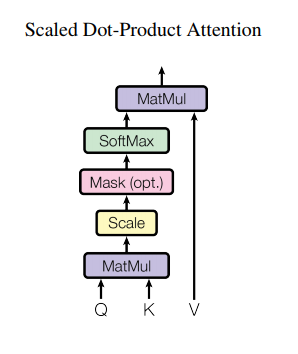
\includegraphics[scale=0.6]{pics/190601-scal.png}}

  

同时论文中提到,将$queries, keys, values$进行h次不同的线性映射,有助于发掘不同的子空间在不同位置上的不同的表示。从而更有益于
最终的模型,Multi-Head的公式化:
$$
			MultiHead(Q, K, V) = Concat(head_1, ..., head_h)W^O 
$$		
$$
			where \; \; head_i = Attention(QW_i^Q, kW_i^K, VW_i^V)
$$
    \centerline{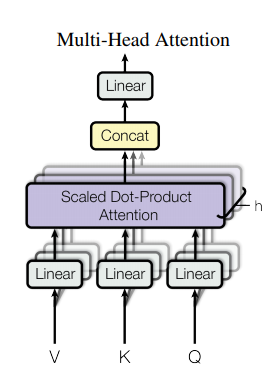
\includegraphics[scale=0.6]{pics/190601-multi.png}}

    
\subsubsection{Self-Attention}

Self Attention 与传统的Attention机制非常的不同:传统的Attention是基于source端和target端的隐含状态(hidden state)
计算Attention的,得到的结果是源端的每个词与目标端每个词之间的依赖关系。

​    但Self Attention不同,它分别在source端和target端进行,仅与source input或者target input自身相关;
捕捉source端或target端\textbf{自身的词与词之间的依赖关系};然后再把source端的得到的self Attention加入到target端得到的Attention中。

 因此,self Attention Attention比传统的Attention mechanism效果要好,主要原因之一是,传统的Attention机制忽略了源端或目标端句子中词与词之间的依赖关系,
相对比,self Attention可以不仅可以得到源端与目标端词与词之间的依赖关系,同时还可以有效获取源端或目标端自身词与词之间的依赖关系:

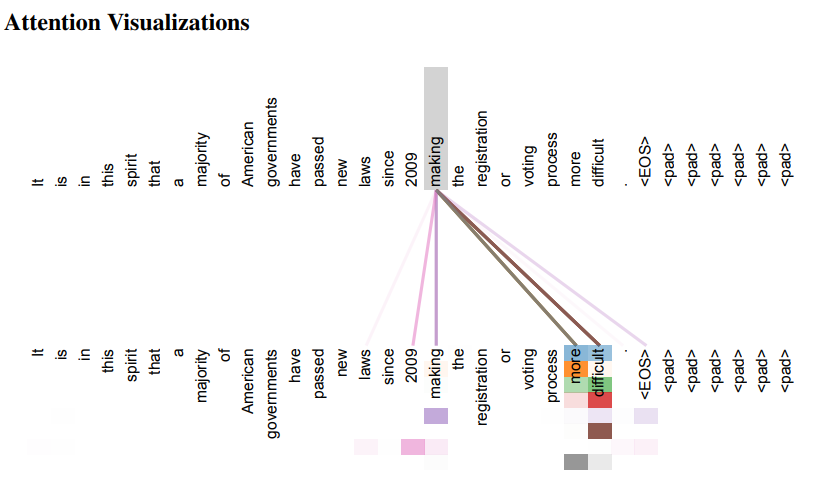
\includegraphics[scale=0.7]{pics/190413-att.png}

\subsection{模型分析}

\subsubsection{模型架构}
Trandformer 将传统模型的Encode,Decoder都换为了多个attention。基本示意图如下:

\begin{figure}
\centering
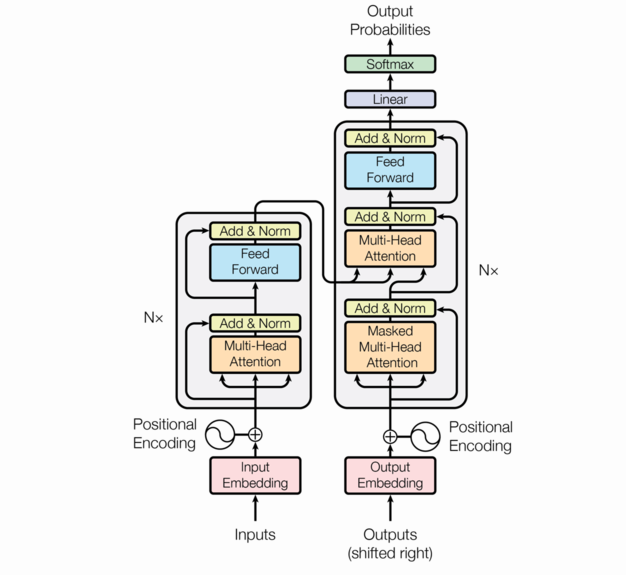
\includegraphics[scale=0.6]{pics/190417-arch.png}
\end{figure}

\begin{itemize}
  \item  左右分别是Encoder和Decoder
  \item Encoder和Decoder的底部是embedding;而embedding又分为两部分:\textbf{input embedding}和\textbf{positional embedding};其中\textbf{input embedding就是seq2seq中的embedding。}
    另一部分是positional embedding,添加该操作是由于transformer中只有attention;而对于attention机制,
    任意一对(query, key)的计算都是完全一样的,不像CNN和RNN,有一个位置或者时序的差异:CNN框住一块区域,随着卷积核移动,
    边缘的少量点会跟着有序变化;RNN更明显了,不同时序的 $h_t$ 和 $s_t$ 不同,而且是随着输入顺序不同(正序,倒序)而不同。
    因此为了体现出时序或者在序列中的位置差异,要对input加入一定的位置信息,即positional embedding。
  \item Encoder 和 Decoder 分别是由N=6 个相同的层叠加得到的。
  \item 对于每一层,Encoder和Decoder的中部分别是两个block,分别输入一个序列、输出一个序列;Encoder的每个block里有两个子层,
    分别是MultiHead Attention和FeedForward Network; Decoder 的block里有三个子层,分别是两个MultiHead Attention和一个FFN。
    这些子网后面都跟了一个add-norm,并且仿照ResNet添加了一个$residual connection$ ,
    对于每一个子层的输出可以形式化表示为$LayerNorm(x + SubLayer(x))$ 也就是子层处理过后的结果加上输入在做正则化处理。
  \item Decoder 的中间的 MultiHead Attention 接受Encoder的输出以及前一个Masked MultiHead Attention 的输出作为输入;
  \item 其中Masked MultiHead Attention是修改过的self-attention, 由于输出的embedding具有一个位置的偏移量,
    使用masking确保了位置i的预测仅取决于小于i的位置处的已知输出。
  \item Decoder最后还有一个Linear和Softmax。
\end{itemize}

\subsubsection{Feed-Forward Network  (FFN)}

基本的前向反馈网络,使用全连接层即可实现。或者使用[1, 1]的卷积实现。使用ReLU作为激活函数。

\centerline{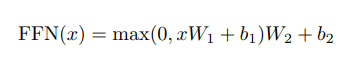
\includegraphics[scale=0.6]{pics/190413-ffn.png}}


\subsubsection{Positional Embedding}

由于网络中没有使用CNN,RNN,为了使用序列的位置信息,必须添加一些额外的信息确定一个token在序列中的相对或者绝对位置。
文中使用的位置编码公式如下:

\centerline{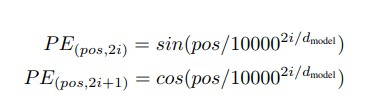
\includegraphics[scale=0.6]{pics/190413-pos.png}}

其中的$pos$是位置,$i$为维度。每一个维度的位置编码为一个正弦曲线,曲线的波长组成了范围在[2$\pi,10000*2\pi$]一个几何级数.
使用这个函数,更容易通过相对位置进行学习,因为对于一个确定的偏差$k$,$PE_{pos+k}$可以使用$PE_{pos}$的线性方程表示。

\setcounter{section}{4}
\section*{四、实验方案}

\setcounter{subsection}{0}
\subsection{数据处理}
  对于 Transformer 的基本架构,使用基于字级别(英文基于word)的模型实现。使用平行语料库进行训练时,对于样本中的每一行$(source, target)$作为一个训练样本,这种方法的主要问题在于难以将具有长距离语义关联的词作为一个样本输入;但是如何发掘语义的关联程度从而确定每一个样本的长度,是一个较为繁琐的工作。所以打算使用一种折中的方式,先使用行粒度的较短样本进行预训练,然后使用多行长样本进一步训练。从而避免了过多预处理的工作。

   由于基于字符进行模型的实现,所以中文分词将每一个字作为最小单元,英文将每一个$word$作为最小单元,对于所有的训练、测试集进行遍历得到所需要的词库。除此之外,对于数据集中出现的标点符号,以及所有有意义的Unicode字符都需要加入到词库中。然后将词库中的所有$item$进行编号,对于每一个句子,可以用一个长度不定的一维向量表示。这样模型的输入就可以用两个一维向量表示。
\subsection{超参设置}
  模型使用前后两套参数进行训练,一个是参数较少的BASE模型,一个是进行预料扩充后的BIG模型.
  \textbf{详细参数见 table1, table2}
  
  \begin{table}[!h]  
    \caption{Base model}  
    \begin{tabularx}{18cm}{lXl}  
      \hline  
      Params & value  & 含义 \\  
    \hline  
    网络参数 \\ \\
    default\_batch\_size  & 512 & 训练时的默认batch \\  
    max\_length & 256 & 最大序列长度 \\
    initializer\_gain & 1.0 & 学习率的初始增益 \\
    vocab\_size & 610,390 & 词库大小 \\
    hidde\_size & 256 & embedding 层的隐含维度\\
    num\_hidden\_layers & 6 & EncoderStack or DecoderStack 的子层数量 \\
    num\_heads & 8 & MultiHead 的head数量 \\
    filter\_size & 1024 & 全连接层的节点数量 \\ 
    
    \\
    丢弃比例 \\ \\ 

    layers\_postprocess\_dropout & 0.1 & 每一层处理后的丢弃比例 \\
    attention\_dropout & 0.1 & attention 层的丢弃比例 \\
    relu\_dropout & 0.1 & 全连接层的丢弃比例 \\

    \\
    train \\  \\
    label\_smoothing & 0.1 & 标记的平滑程度 \\
    learning\_rate & 2.0 & 学习率 \\
    learning\_rate\_deacy\_rate & 1.0 & 学习率的衰减率 \\
    learning\_rate\_warmup\_steps & 16000 & lr 平方根倒数衰减的初始值 \\
    train\_steps & 100000 & 训练步数 \\
    steps\_between\_evals & 5000 & evaluate 间隔步数 \\
    eval\_step & 25 & evaluate 步数 \\ 
        
    \\
    optimizer \\ \\ 
    optimizer\_adam_beta1 & 0.9 & adam 梯度下降参数1 \\
    optimizer\_adam_beta2 & 0.997 & adam 梯度下降参数2 \\ 

    \\
    predict \\ \\
    extra\_decode\_length & 50 & 额外编码长度 \\ 
    beam\_size & 4 & beam search 的参数 \\
    alpha & 0.6 & beam search 参数 \\
    \hline

    \end{tabularx} 
  \end{table}  
  
  \begin{table}[!h]
    \caption{Big Model}
      \begin{tabularx}{18cm}{lXl}
      \hline
      Params & value  & 含义 \\
      \hline
      *仅记录与Base Model不同的参数 \\
      \hline
        vocab\_size  & 1132998 & 词库大小 \\
        hidden\_size  & 128 & Embedding 隐含维度 \\
      \hline
    \end{tabularx}
  \end{table}
  

  
\subsection{优化函数}
  模型使用的 Adam Oprtimizer, 对应的参数 $\beta_1 = 0.9$, $beta = 0.98$. 为了降低过拟合风险,在训练过程中进行
  学习率的衰减, 衰减公式如下:

  $$
    lrate = d_{model} ^{-0.5} * min(step_num^{-0.5}, step_num * warmup_steps ^{-1.5})
  $$

  在前$warmup_steps$ 学习率线性增长, 当到达该阈值后,开始训练步数的平方根的倒数进行衰减.

\subsection{正则化}

\subsubsection{Residual Drouout}
在Encoder Stack(Decoder Stack)每一个子层的输出上进行dropout, 然后再加上该层的输入, 再进行正则化(BatchNormal).
所以实现residual 的结构.
除此之外,在模型的输入上,对于embedding以及positional encoding的和也进行了drpout. 使用的dropout比例为0.1.



\setcounter{section}{5}
\section*{五、实验结果}

\setcounter{subsection}{0}
\subsection{评价指标}
\subsubsection{BLEU}
\textbf{BLEU (bilingual evaluation understudy)} 是机器翻译中最常用的评价指标. 将机器翻译的输出与人工翻译进行比较,作为模型质量的评估.
BLEU的输出始终是介于0和1之间的数字。此值表示候选文本与参考文本的相似程度,值接近1表示更相似的文本。很少有人类翻译得分为1,因为这表明候选人与其中一个参考译文相同。因此,没有必要获得1分。因为有更多的机会匹配,添加额外的参考翻译将增加BLEU分数.

使用n-gram的BLEU作为评价指标:
  $$
    Count_{w_i, j}^{clip} = min(Count_{w_i}, Ref_j-Count_{w_i})
  $$

  $$
    Count^{clip} = max(Count_{w_i, j}^{clip}) 
  $$
  
  $$
    BLEU_{n} = \frac{Count^{clip}}{n}
  $$

  \begin{tcolorbox}
  \begin{itemize}
      \item $Count_{W_i}$: 翻译结果中单词$w_i$的数量
      \item $Ref_j-Count_{w_i}$: 单词$w_i$在第j个参考翻译中的数量
      \item $Count_{W_i, j}$: 单词$w_i$在第j个参考翻译中的截断计数
      \item $Count^{clip}$: 单词$w_i$在所有参考翻译中的截断计数
      \item $BLEU_n$: n-gram 下的BLEU值
  \end{itemize}
\end{tcolorbox}

  本实验的验证主要是基于 BLEU\_4这一指标。



\subsection{结果}
\begin{tabular}{ccc}
  \hline
  实现 & BLEU\_4 (*0.01) & 语料库 \\
  \hline
  Transformer (Our Imple) & 15 & UMCORPUS \\
  Transformer (THUMT Imple) & 34 & EN-DE(WMT-17) \\
  Transformer (Paper Imple) & 28.5 & EN-DE(WMT-14) \\  
  \hline
\end{tabular}

\setcounter{section}{6}
\section*{六、团队分工}

\begin{tabular}{ccc}
  \hline
  姓名& 学号& 任务\\
  \hline
  贾栋&201600301129 &Transformer 模型的搭建,并在此基础上改进;实验报告的书写\\
  王坤&201600301225 &数据的收集与整理;三大开源模型的源码分析,以及模型比对\\
  \hline
\end{tabular}

\setcounter{section}{7}
\section*{七、总结以及未来工作}

\setcounter{subsection}{0}
\subsection{主要收获与思考}
  本次NLP实验,针对机器翻译的任务,对于Transformer基本模型进行了实现。主要对于模型的主体架构、核心算法、创新之处进行了详细分析;在具体实现过程中,
  遇到了不同的问题,尤其在数据处理、训练时调参等方面仍有不足之处。但是总体来说收获颇丰,一方面从Seq2seq模型出发,对于序列翻译,attention机制,有了实际的
  认知与把握;另一方面,Transformer模型对于基本Seq2seq的结构创新,也给了我很大的启发,放弃惯有的CNN、RNN,仅仅使用attention机制,该模型单从创意来说就是
  一次不错的尝试,而且从结果来说,在特定任务上获得了更为优异的性能,并且启发了与之相关的其他工作。不得不说,这是一项优秀的工作。

  在实现方面,利用Tensorflow API, 虽然论文中对于模型的结构,基本的原理有了较为明确的阐释,并且给出了一些训练时的超参数。但是在具体实现过程中仍有一定的难度。
  一方面需要对于API掌握较为熟练,另一方面需要仔细分析每一部分的具体组织形式。虽然遇到了很多Bug, 需要处理很多与模型无关的繁琐工作,最后还是得到了所需要的程序。
  在实现过程中,通过不断查阅文档,加深了对Tensorflow框架的基本API的掌握,同时了解了一些高级用法,比如 \textmd{`tf.estimator`} 模块等。
  从中也受益匪浅。

\subsubsection{不足之处}
在数据领域一致认为:数据和特征决定了机器学习的上限,而模型和算法只能逼近这个上限而已。本次实验,我对于这个说法深有感触。由于数据处理方面经验的不足,
面对大量的数据时,没有一个鲁棒的、可扩展的数据处理方法。导致了相同的模型,我在实际操作时,不管是具体的翻译结果还是各项评价指标都与论文所述存在较大差距。
放下模型实现过程中可能的缺陷不说,但就分词一项,就决定了最终模型的性能上限。最初的模型是基于学长给的语料库,进行简单的基于字符级别的分词,词典大小为610,390;
基本的分词结果尚且可行;但是后续语料库的扩充,出现了较大问题,单就英文来说,很多词由于没有空格隔开,导致分为一个词, 例如: \textbf{positiveinjunctions
, people'opinions, indistinguishable51, MockStrutsTestCase.. 除此之外,词库中还有一些无意义的词。}下面是部分词库内容截图:

\centerline{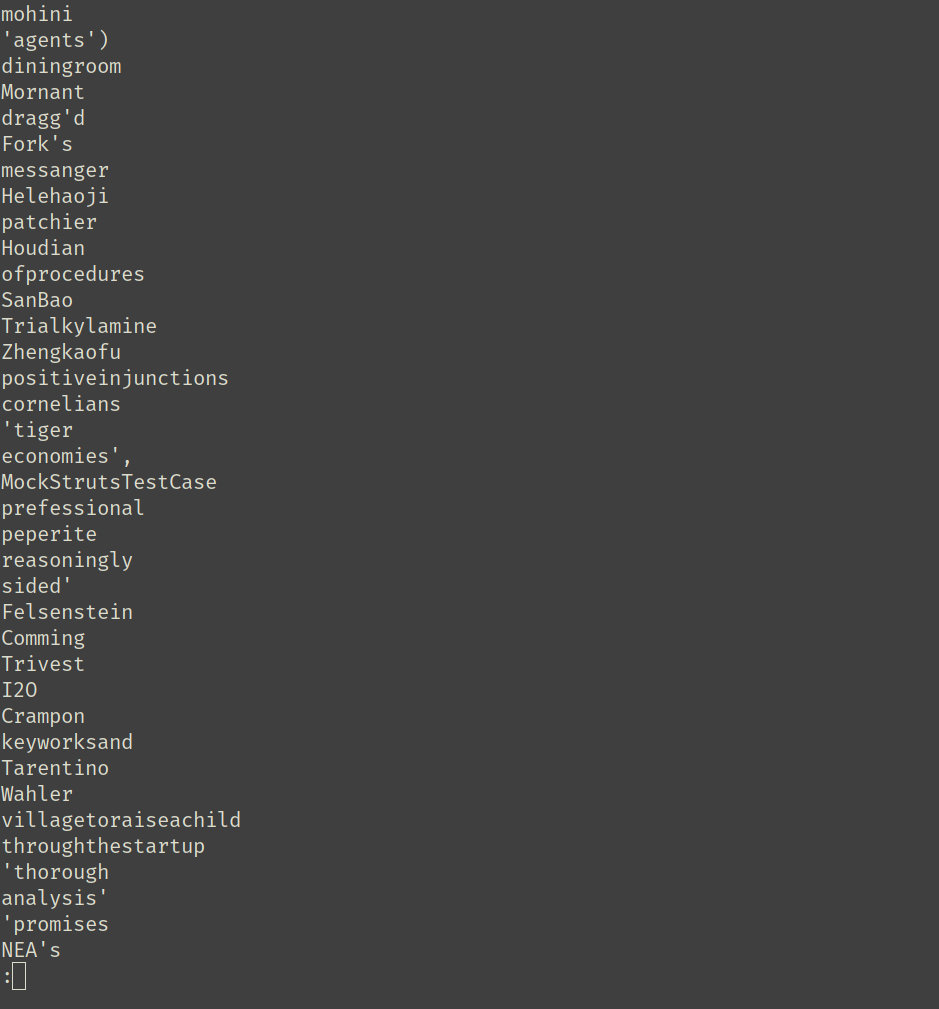
\includegraphics[scale=0.5]{pics/190605-vocab.png}}

造成这种情形的主要原因是对于可能存在异常的example没有进行滤出。除此之外,还有一个最大的问题是,实验将每一行的中英翻译作为一个训练样例,这样做虽然操作简单,
但是实际情形是,翻译并不一定是单行对应的,这样的实现没有将一个具有完整的语义的翻译作为一个训练样例, 得到的结果也就存在较大问题。同时,基于字符级别的分词,具有一个显著的缺陷 ---- \textbf{进行语料库扩充时
, 词典也会随之扩充,那么原有的训练工作就完全浪费了,因为模型的第一个Embedding层的参数数量与词库大小相关,这样,模型就不具备可扩展性。}所以,我的实现还是存在致命错误的。
主要原因在于,在工作之初没有制定一个可扩展的数据方案,以及合理的分词规则。
\subsection{未来工作}
首先是对现有实现的改进,主要从数据处理、模型的可扩展方面进行。

对于平行语料库,关键在于找到一个准确的具有完整语义的句子作为一个训练样本。单纯使用基于标点符号的划分并不准确,这样得到的模型缺乏对于长语义关联的辨识度。
目前还没有较好的解决方案。对于词典的可扩展性问题,可以使用subtoken的方式,一个词用其子结构表示,词典只存储子结构,这样进行编码时,每一个词可以用一个整形列表表示。
例如: \textbf{example: 它的子结构可能是exam, ple, 对于词典编号 [12, 22], 这样exmaple的编码为[12, 22, 0], 0为词结束标志}。这样,只要记录子结构,每一个词都可以
作为一个列表表示,就不需要扩充词典。对于中文的表示,暂无好的想法。

在对Transformer模型的数据、模型进行完善之后,可以对于其他基于Transformer的工作进行复现。
\section*{八、参考文献}
\href{https://arxiv.org/pdf/1409.0473.pdf}{\color{blue}Bahadanau attention}

\href{https://arxiv.org/pdf/1706.03762.pdf}{\color{blue}Attention is all you need}

\href{https://arxiv.org/pdf/1808.09381.pdf}{\color{blue}https://arxiv.org/pdf/1808.09381.pdf}

\href{https://www.aclweb.org/anthology/P02-1040.pdf}{\color{blue} BLEU: a Method for Automatic Evaluation of Machine Translation}

\href{https://www.aclweb.org/anthology/W04-1013}{\color{blue} ROUGE: A Package for Automatic Evaluation of Summaries}

\href{https://www.tensorflow.org/api_docs/python/tf}{\color{blue} Tensorflow API}

\href{https://zhuanlan.zhihu.com/p/38485843}{\color{blue}https://zhuanlan.zhihu.com/p/3848584}

\href{https://juejin.im/entry/5a1f9e036fb9a0450671663c}{\color{blue}https://juejin.im/entry/5a1f9e036fb9a0450671663c}



\end{document}
